\documentclass[tikz,border=7pt]{standalone}
% Shared TikZ style for the Nios V stereo accelerator diagrams.
\usepackage[T1]{fontenc}
\usepackage{lmodern}
\usepackage{xcolor}
\usepackage{tikz}
\usetikzlibrary{arrows.meta,backgrounds,calc,fit,positioning}

\definecolor{navy}{HTML}{073D73}
\definecolor{blue}{HTML}{0B5CAB}
\definecolor{cyan}{HTML}{1B8DBB}
\definecolor{green}{HTML}{27845B}
\definecolor{orange}{HTML}{C66A16}
\definecolor{red}{HTML}{B94444}
\definecolor{ink}{HTML}{172033}
\definecolor{muted}{HTML}{5A6678}
\definecolor{line}{HTML}{BFCBDA}
\definecolor{softblue}{HTML}{EDF4FA}
\definecolor{softcyan}{HTML}{ECF8FB}
\definecolor{softgreen}{HTML}{EEF8F2}
\definecolor{softorange}{HTML}{FFF4E8}
\definecolor{softgray}{HTML}{F5F7FA}

% Avoid automatic word hyphenation inside compact diagram nodes.
\hyphenpenalty=10000
\exhyphenpenalty=10000

\tikzset{
  font=\sffamily,
  block/.style={
    draw=line, rounded corners=2.2pt, fill=white,
    minimum height=10mm, text width=31mm, align=center,
    inner xsep=3mm, inner ysep=2.2mm
  },
  cpu/.style={block, draw=blue!55, fill=softblue},
  accel/.style={block, draw=cyan!65, fill=softcyan},
  memory/.style={block, draw=green!60, fill=softgreen},
  control/.style={block, draw=orange!65, fill=softorange},
  smallblock/.style={block, text width=24mm, minimum height=8mm, inner xsep=2mm, inner ysep=1.6mm},
  group/.style={draw=line, rounded corners=4pt, fill=softgray, inner sep=4mm},
  labeltag/.style={rounded corners=2pt, fill=navy, text=white, font=\sffamily\bfseries\footnotesize, inner xsep=2.5mm, inner ysep=1.2mm},
  flow/.style={-{Stealth[length=2.6mm,width=1.8mm]}, draw=navy, line width=0.85pt},
  dataflow/.style={-{Stealth[length=2.8mm,width=2mm]}, draw=blue, line width=1.15pt},
  controlflow/.style={-{Stealth[length=2.4mm,width=1.7mm]}, draw=orange, line width=0.9pt, dashed},
  returnflow/.style={-{Stealth[length=2.4mm,width=1.7mm]}, draw=green, line width=0.9pt},
  bus/.style={<->, >={Stealth[length=2.8mm,width=2mm]}, draw=navy, line width=1.6pt},
  note/.style={font=\sffamily\footnotesize, text=muted, align=left},
  arrowlabel/.style={font=\sffamily\scriptsize, text=muted, fill=white, inner sep=1.2pt}
}


\begin{document}
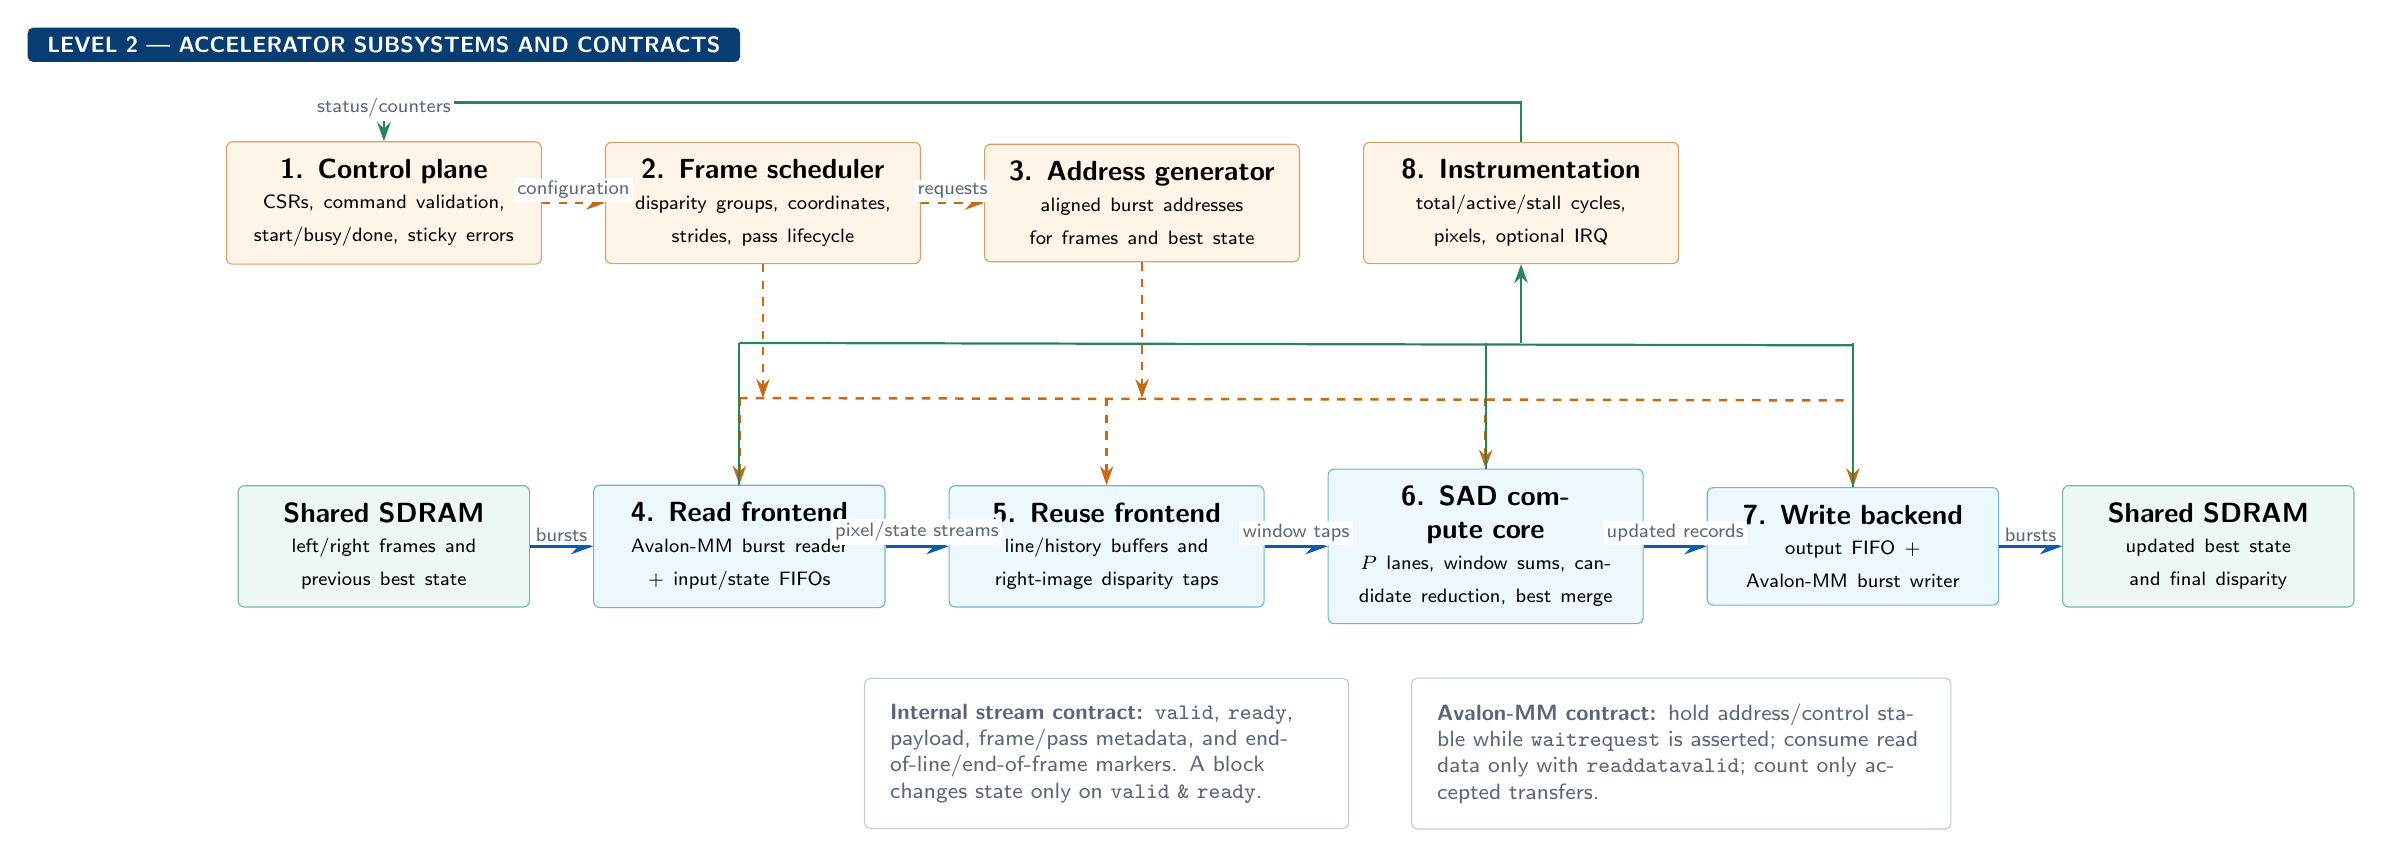
\begin{tikzpicture}[node distance=8mm and 8mm]
  \node[labeltag] (title) {LEVEL 2 --- ACCELERATOR SUBSYSTEMS AND CONTRACTS};

  \node[control, text width=34mm, below=10mm of title] (csr) {\textbf{1. Control plane}\\[-1pt]\scriptsize CSRs, command validation, start/busy/done, sticky errors};
  \node[control, text width=34mm, right=8mm of csr] (sched) {\textbf{2. Frame scheduler}\\[-1pt]\scriptsize disparity groups, coordinates, strides, pass lifecycle};
  \node[control, text width=34mm, right=8mm of sched] (addr) {\textbf{3. Address generator}\\[-1pt]\scriptsize aligned burst addresses for frames and best state};
  \node[control, text width=34mm, right=8mm of addr] (perf) {\textbf{8. Instrumentation}\\[-1pt]\scriptsize total/active/stall cycles, pixels, optional IRQ};

  \node[memory, text width=31mm, below=28mm of csr] (sdramIn) {\textbf{Shared SDRAM}\\[-1pt]\scriptsize left/right frames and previous best state};
  \node[accel, text width=31mm, right=8mm of sdramIn] (read) {\textbf{4. Read frontend}\\[-1pt]\scriptsize Avalon-MM burst reader + input/state FIFOs};
  \node[accel, text width=34mm, right=8mm of read] (reuse) {\textbf{5. Reuse frontend}\\[-1pt]\scriptsize line/history buffers and right-image disparity taps};
  \node[accel, text width=34mm, right=8mm of reuse] (compute) {\textbf{6. SAD compute core}\\[-1pt]\scriptsize $P$ lanes, window sums, candidate reduction, best merge};
  \node[accel, text width=31mm, right=8mm of compute] (write) {\textbf{7. Write backend}\\[-1pt]\scriptsize output FIFO + Avalon-MM burst writer};
  \node[memory, text width=31mm, right=8mm of write] (sdramOut) {\textbf{Shared SDRAM}\\[-1pt]\scriptsize updated best state and final disparity};

  \draw[dataflow] (sdramIn) -- node[arrowlabel, above] {bursts} (read);
  \draw[dataflow] (read) -- node[arrowlabel, above] {pixel/state streams} (reuse);
  \draw[dataflow] (reuse) -- node[arrowlabel, above] {window taps} (compute);
  \draw[dataflow] (compute) -- node[arrowlabel, above] {updated records} (write);
  \draw[dataflow] (write) -- node[arrowlabel, above] {bursts} (sdramOut);

  \draw[controlflow] (csr) -- node[arrowlabel, above] {configuration} (sched);
  \draw[controlflow] (sched) -- node[arrowlabel, above] {requests} (addr);
  \coordinate (controlbusL) at ($(read.north)+(0,11mm)$);
  \coordinate (controlbusR) at ($(write.north)+(0,11mm)$);
  \draw[draw=orange, dashed, line width=.9pt] (controlbusL) -- (controlbusR);
  \draw[controlflow] (sched.south) -- (sched.south |- controlbusL);
  \draw[controlflow] (addr.south) -- (addr.south |- controlbusL);
  \foreach \child in {read,reuse,compute,write} {
    \draw[controlflow] (\child.north |- controlbusL) -- (\child.north);
  }

  \coordinate (eventbusL) at ($(read.north)+(0,18mm)$);
  \coordinate (eventbusR) at ($(write.north)+(0,18mm)$);
  \draw[draw=green, line width=.8pt] (eventbusL) -- (eventbusR);
  \foreach \source in {read,compute,write} {
    \draw[draw=green, line width=.8pt] (\source.north) -- (\source.north |- eventbusL);
  }
  \draw[returnflow] (perf.south |- eventbusL) -- (perf.south);
  \draw[returnflow] (perf.north) -- ++(0,5mm) -| node[arrowlabel, near end, above] {status/counters} (csr.north);

  \node[note, text width=55mm, below=11mm of reuse] (streamif) {\textbf{Internal stream contract:} \texttt{valid}, \texttt{ready}, payload, frame/pass metadata, and end-of-line/end-of-frame markers. A block changes state only on \texttt{valid \& ready}.};
  \node[note, text width=62mm, right=12mm of streamif] (busif) {\textbf{Avalon-MM contract:} hold address/control stable while \texttt{waitrequest} is asserted; consume read data only with \texttt{readdatavalid}; count only accepted transfers.};
  \draw[draw=line, rounded corners=2pt] ([xshift=-2mm,yshift=-2mm]streamif.south west) rectangle ([xshift=2mm,yshift=2mm]streamif.north east);
  \draw[draw=line, rounded corners=2pt] ([xshift=-2mm,yshift=-2mm]busif.south west) rectangle ([xshift=2mm,yshift=2mm]busif.north east);
\end{tikzpicture}
\end{document}
